\section{Date: 2026-09-24}
\noindent \textbf{Series ID: SWSTFRBCIRGSP} 

\noindent This series is titled Real Gross Domestic Product: Monetary Authorities-Central Bank, Credit Intermediation, and Related Services (521-522) in the Southwest BEA Region and has a frequency of Annual. The units are Millions of Chained 2017 Dollars and the seasonal adjustment is Not Seasonally Adjusted.The observation start date is 1997-01-01 and the observation end date is 2024-01-01.The popularity of this series is 1. \\ 

\noindent \textbf{Series ID: LLRNPT39} 

\noindent This series is titled Assets at Banks whose ALLL exceeds their Nonperforming Loans, Banks with Total Assets from \$1B to \$10B, Pacific Census Division (DISCONTINUED) and has a frequency of Quarterly, End of Period. The units are Percent and the seasonal adjustment is Not Seasonally Adjusted.The observation start date is 1988-01-01 and the observation end date is 2020-07-01.The popularity of this series is 1. \\ 

\subsection{Raw Regression}
\noindent Regresses the two series against each other directly. A significant result here can come just as easily from both series sharing a long-run trend as from any real relationship.

\begin{center}
\begin{tabular}{lclc}
\toprule
\textbf{Dep. Variable:}             & value\_fred\_LLRNPT39 & \textbf{  R-squared:         } &     0.158   \\
\textbf{Model:}                     &          OLS          & \textbf{  Adj. R-squared:    } &     0.119   \\
\textbf{Method:}                    &     Least Squares     & \textbf{  F-statistic:       } &     4.120   \\
\textbf{Date:}                      &    Thu, 24 Sep 2026   & \textbf{  Prob (F-statistic):} &   0.0546    \\
\textbf{Time:}                      &        15:59:56       & \textbf{  Log-Likelihood:    } &   -110.56   \\
\textbf{No. Observations:}          &             24        & \textbf{  AIC:               } &     225.1   \\
\textbf{Df Residuals:}              &             22        & \textbf{  BIC:               } &     227.5   \\
\textbf{Df Model:}                  &              1        & \textbf{                     } &             \\
\textbf{Covariance Type:}           &       nonrobust       & \textbf{                     } &             \\
\bottomrule
\end{tabular}
\begin{tabular}{lcccccc}
                                    & \textbf{coef} & \textbf{std err} & \textbf{t} & \textbf{P$> |$t$|$} & \textbf{[0.025} & \textbf{0.975]}  \\
\midrule
\textbf{const}                      &     152.7995  &       40.101     &     3.810  &         0.001        &       69.635    &      235.964     \\
\textbf{value\_fred\_SWSTFRBCIRGSP} &      -0.0016  &        0.001     &    -2.030  &         0.055        &       -0.003    &     3.37e-05     \\
\bottomrule
\end{tabular}
\begin{tabular}{lclc}
\textbf{Omnibus:}       &  4.915 & \textbf{  Durbin-Watson:     } &    0.325  \\
\textbf{Prob(Omnibus):} &  0.086 & \textbf{  Jarque-Bera (JB):  } &    3.660  \\
\textbf{Skew:}          & -0.955 & \textbf{  Prob(JB):          } &    0.160  \\
\textbf{Kurtosis:}      &  3.111 & \textbf{  Cond. No.          } & 4.07e+05  \\
\bottomrule
\end{tabular}
%\caption{OLS Regression Results}
\end{center}

Notes: \newline
 [1] Standard Errors assume that the covariance matrix of the errors is correctly specified. \newline
 [2] The condition number is large, 4.07e+05. This might indicate that there are \newline
 strong multicollinearity or other numerical problems.

\begin{figure}
\centering
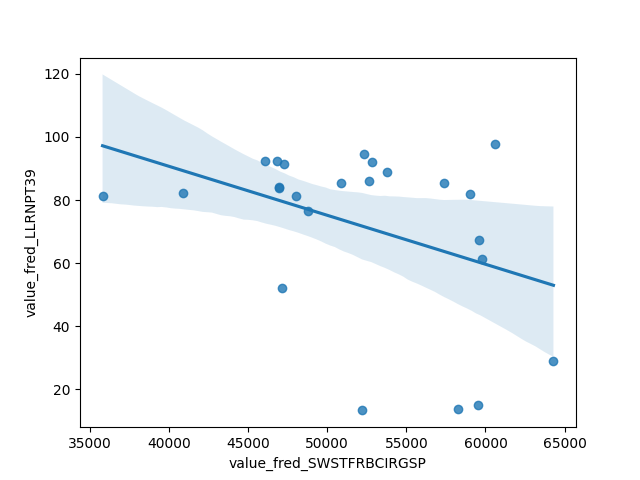
\includegraphics[scale = 0.9]{plots/plot_2026-09-24.png}
\caption{Raw Regression Plot for 2026-09-24}
\end{figure}
\newpage
\subsection{Detrended Regression}
\noindent Regresses the residuals of each series after removing its own linear time trend, so a shared trend can no longer drive the result on its own. A relationship that stays significant here is better evidence of a genuine link between the two series.

\begin{center}
\begin{tabular}{lclc}
\toprule
\textbf{Dep. Variable:}                        & value\_fred\_LLRNPT39\_detrended & \textbf{  R-squared:         } &     0.277   \\
\textbf{Model:}                                &               OLS                & \textbf{  Adj. R-squared:    } &     0.244   \\
\textbf{Method:}                               &          Least Squares           & \textbf{  F-statistic:       } &     8.412   \\
\textbf{Date:}                                 &         Thu, 24 Sep 2026         & \textbf{  Prob (F-statistic):} &  0.00830    \\
\textbf{Time:}                                 &             15:59:56             & \textbf{  Log-Likelihood:    } &   -108.67   \\
\textbf{No. Observations:}                     &                  24              & \textbf{  AIC:               } &     221.3   \\
\textbf{Df Residuals:}                         &                  22              & \textbf{  BIC:               } &     223.7   \\
\textbf{Df Model:}                             &                   1              & \textbf{                     } &             \\
\textbf{Covariance Type:}                      &            nonrobust             & \textbf{                     } &             \\
\bottomrule
\end{tabular}
\begin{tabular}{lcccccc}
                                               & \textbf{coef} & \textbf{std err} & \textbf{t} & \textbf{P$> |$t$|$} & \textbf{[0.025} & \textbf{0.975]}  \\
\midrule
\textbf{const}                                 &    1.199e-12  &        4.776     &  2.51e-13  &         1.000        &       -9.904    &        9.904     \\
\textbf{value\_fred\_SWSTFRBCIRGSP\_detrended} &      -0.0031  &        0.001     &    -2.900  &         0.008        &       -0.005    &       -0.001     \\
\bottomrule
\end{tabular}
\begin{tabular}{lclc}
\textbf{Omnibus:}       &  7.727 & \textbf{  Durbin-Watson:     } &    0.515  \\
\textbf{Prob(Omnibus):} &  0.021 & \textbf{  Jarque-Bera (JB):  } &    5.892  \\
\textbf{Skew:}          & -1.175 & \textbf{  Prob(JB):          } &   0.0526  \\
\textbf{Kurtosis:}      &  3.608 & \textbf{  Cond. No.          } & 4.43e+03  \\
\bottomrule
\end{tabular}
%\caption{OLS Regression Results}
\end{center}

Notes: \newline
 [1] Standard Errors assume that the covariance matrix of the errors is correctly specified. \newline
 [2] The condition number is large, 4.43e+03. This might indicate that there are \newline
 strong multicollinearity or other numerical problems.

\begin{figure}
\centering
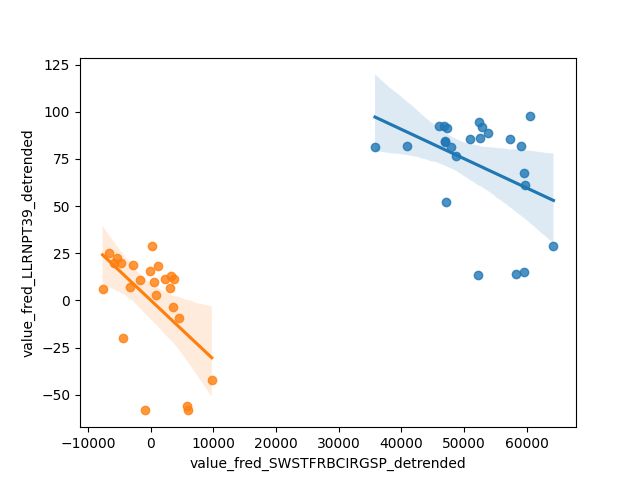
\includegraphics[scale = 0.9]{plots/plot_2026-09-24_detrended.png}
\caption{Detrended Regression Plot for 2026-09-24}
\end{figure}
\newpage
